\subsection{Fonctionnalité 5}
La fonctionnalité 5 permettra d'afficher une carte montrant les lieux où des demandes d'intervention ont été faites pour un créneau que l'utilisateur aura entré.
La figure \ref{maquetteCarteIntervention} présente une maquette de la carte des interventions.

% Figure : version 1.00, date 24/02/16, auteur Mélissa Bignoux
\begin{figure}[H]
	\centering
	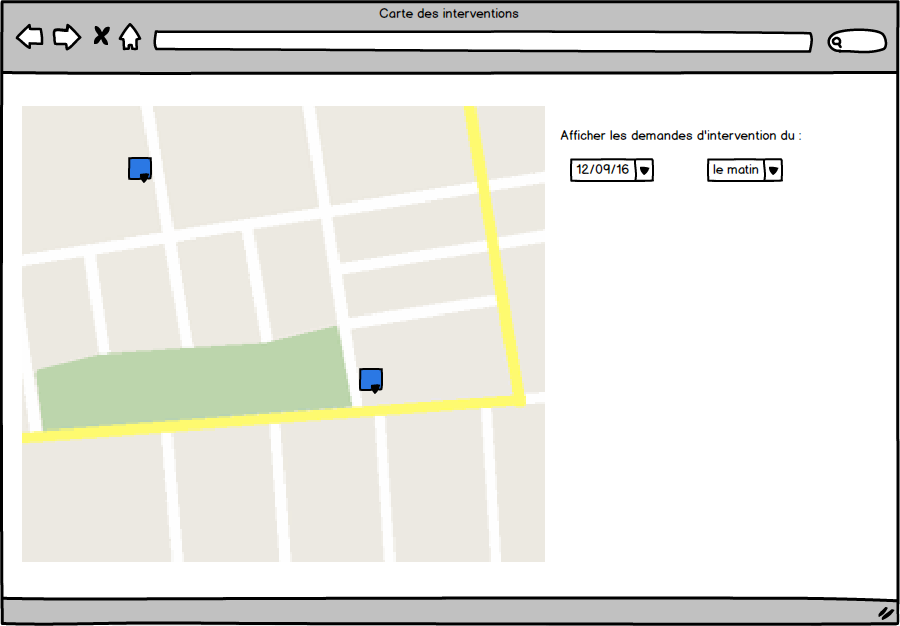
\includegraphics[scale=0.575]{images/maquettes/fonctionnalite5CarteDesInterventions.png}
	\caption{Maquette~: Carte des interventions en fonction d'une date choisie et du moment de la journée}
	\label{maquetteCarteIntervention}
\end{figure}

La fonctionnalité 5 consistera également à planifier les interventions c'est-à-dire qu'un plaideur s'attribue une intervention.
Lors de chaque affectation, un e-mail d'information de prise en charge de la demande par l'équipe de plaideur sera envoyé à l'établissement demandeur ainsi qu'au responsable de l'activité demandée.
Une intervention ne peut être attribuée qu'à un utilisateur.
\\

\begin{figure}[H]
	\centering
	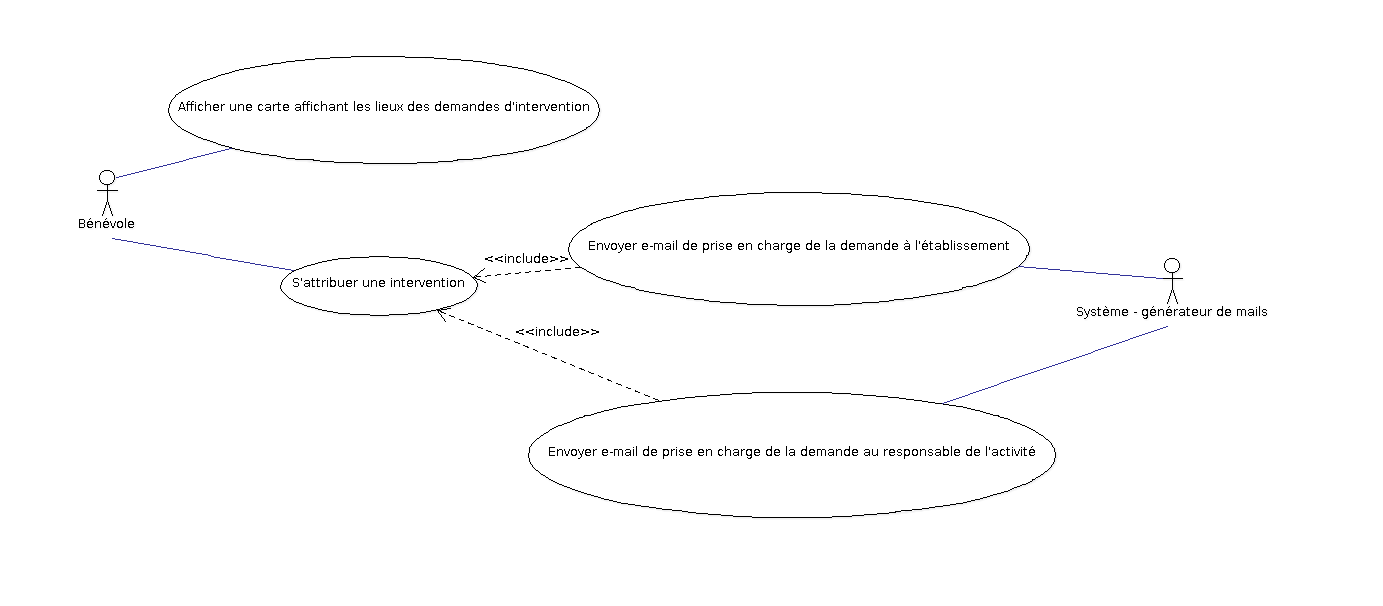
\includegraphics[scale=0.4]{images/casDUtilisation/fonctionnalite5Attribution.png}
	 \caption{Cas d'utilisation~: Visualiser les demandes et s'attribuer des interventions}
	 \label{visualiserESAttribuer}
\end{figure}

% Figure : version 1.00, date 24/02/16, auteur Michel Cressant
\begin{figure}[H]
	\centering
	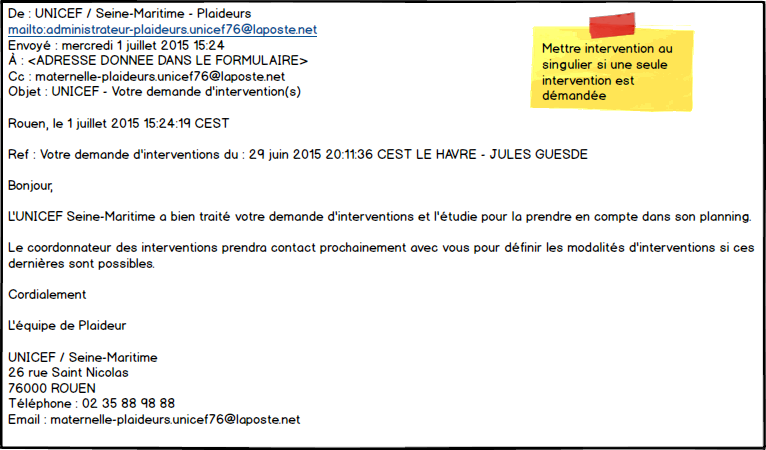
\includegraphics[scale=0.675]{images/maquettes/fonctionnalite5MailDePriseEnCharge.png}
	\caption{Maquette~: Email de prise en charge d'une intervention}
\end{figure}
